\begingroup
\shorthandoff{=}
\renewcommand{\tablename}{Tablo}
\renewcommand{\figurename}{Şekil}
\graphicspath{{src/figures/}{figures/}}

\section{Sonuçların analizi}
\label{sec:benchmark-analysis}

\subsection{Nitel analiz}
WO'nun nitel sonuçları, standart kıyaslama fonksiyonları kullanılarak
değerlendirilmiştir. İncelenen kıyaslama kümesi, fonksiyonların optimizasyon
yapısına ve boyut özelliklerine göre üç gruba ayrılmıştır:
tek tepeli (unimodal), çok tepeli (multimodal) ve sabit boyutlu çok tepeli
(fixed-dimension multimodal) fonksiyonlar. Makale \cite{han2024walrus}’te önerilen 
bu sınıflandırmaya göre F1–F7 fonksiyonları tek tepeli, F8–F13 fonksiyonları çok tepeli, 
F14–F23 fonksiyonları ise sabit boyutlu çok tepeli grupta yer almaktadır.
\cite{han2024walrus}.

Tek tepeli fonksiyonlar tek bir küresel optimuma sahiptir. Bu nedenle,
algoritmanın optimuma doğru ilerlemesi ve çözüm kalitesini iyileştirmesi
hakkında bilgi verirler. Çok tepeli fonksiyonlar birden fazla yerel optimum
içerir; bu fonksiyonlar algoritmanın yerel çözümlere erken yakınsama
eğilimini ve arama uzayının farklı bölgelerini keşfetme yeteneğini incelemek
için kullanılır. Sabit boyutlu çok tepeli fonksiyonlarda ise değişken sayısı
fonksiyonun tanımıyla belirlenmiştir ve keyfî olarak artırılamaz. Bu grup,
algoritmanın belirli boyutlara sahip, daha karmaşık ve çok tepeli arama
uzaylarındaki davranışını değerlendirmeye olanak tanır.

Sonuçlar dört ölçüt üzerinden incelenmiştir: arama geçmişi, ilk ajanın
yörüngesi, popülasyonun ortalama uygunluğu ve yakınsama eğrisi
\cite{han2024walrus}. Arama geçmişi, ajanların iterasyonlar boyunca ziyaret
ettiği bölgeleri; ilk ajanın yörüngesi, tek bir ajanın hareketini; ortalama
uygunluk, popülasyonun genel performansını; yakınsama eğrisi ise iterasyonlar
boyunca elde edilen en iyi çözümün değişimini gösterir. Böylece WO'nun hem
arama uzayını keşfetme davranışı hem de çözümleri iyileştirme süreci nitel
olarak değerlendirilebilir.

\begin{figure}[htbp]
\centering
\begin{minipage}[t]{0.48\textwidth}\centering\small
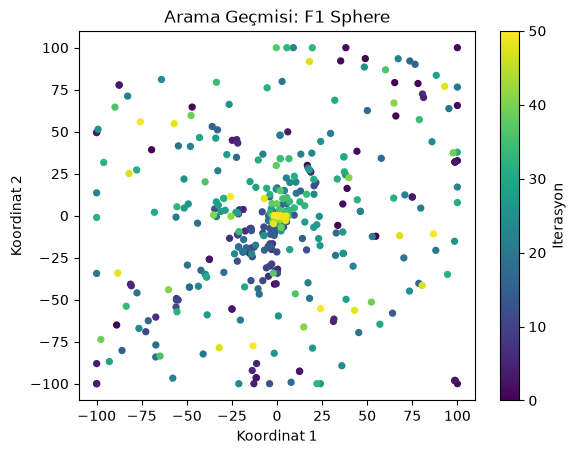
\includegraphics[width=\linewidth]{F1/search_history.png}
\end{minipage}\hfill
\begin{minipage}[t]{0.48\textwidth}\centering\small 
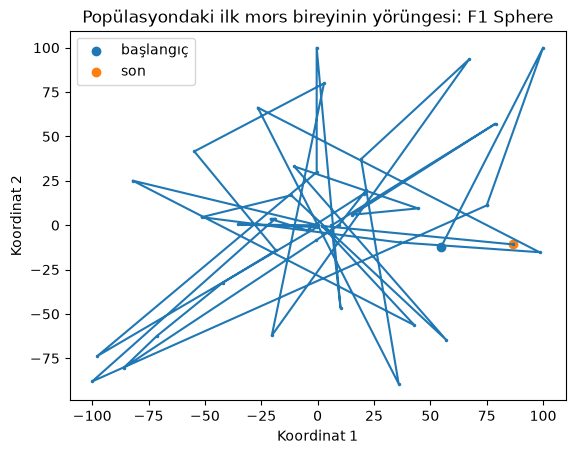
\includegraphics[width=\linewidth]{F1/first_walrus_trajectory.png}
\end{minipage}\par\medskip
\begin{minipage}[t]{0.48\textwidth}\centering\small
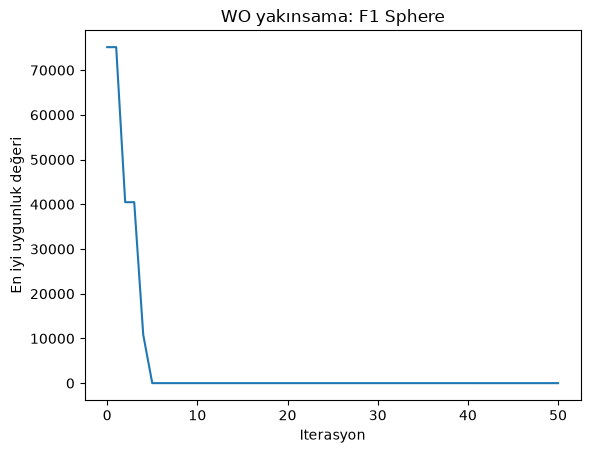
\includegraphics[width=\linewidth]{F1/convergence.png}
\end{minipage}\hfill
\begin{minipage}[t]{0.48\textwidth}\centering\small
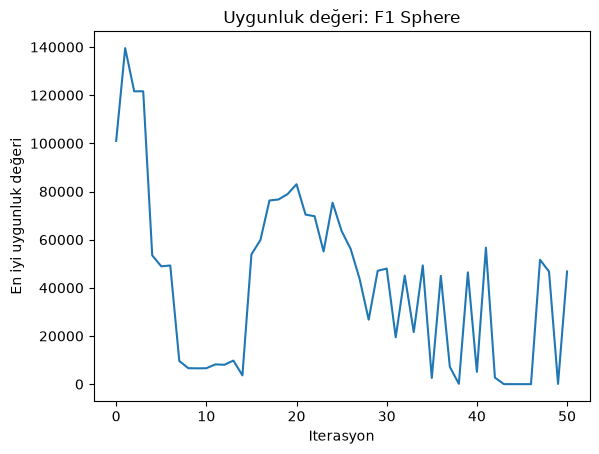
\includegraphics[width=\linewidth]{F1/average_fitness.png}
\end{minipage}
\caption{WO'nun F1 Sphere fonksiyonundaki nitel arama sonuçları.}
\label{fig:wo-f1-qualitative}
\end{figure}

Şekil~\ref{fig:wo-f1-qualitative}'de arama geçmişinin önemli bir bölümü optimum olan orijinin çevresinde 
yoğunlaşırken arama uzayına yayılan sıçramalar da görülmektedir. İlk morsun yörüngesi geniş ve ani hareketler içerir; 
yörüngenin son noktası optimuma yakın değildir. Buna karşın, yakınsama eğrisi en iyi uygunluğun ilk birkaç yinelemede sıfıra 
yaklaştığını ve sonrasında korunduğunu gösterir. Popülasyonun ortalama uygunluğu ise yinelemeler boyunca belirgin biçimde 
dalgalanır. 

\begin{figure}[htbp]
\centering
\begin{minipage}[t]{0.48\textwidth}\centering\small
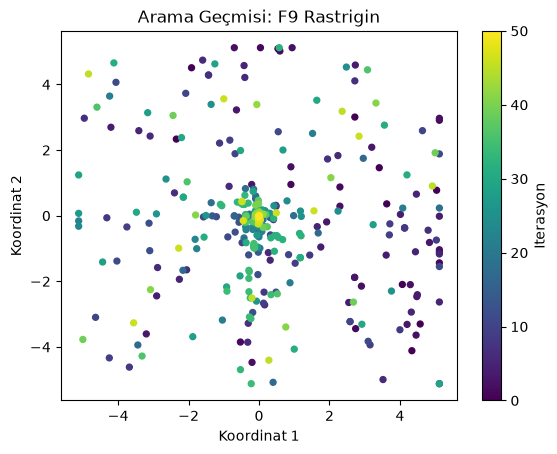
\includegraphics[width=\linewidth]{F9/search_history.png}
\end{minipage}\hfill
\begin{minipage}[t]{0.48\textwidth}\centering\small 
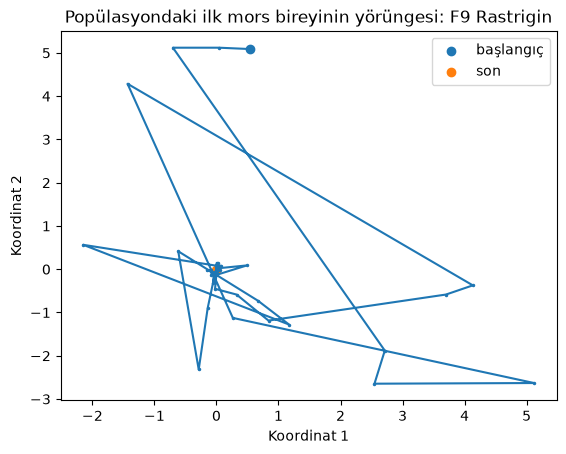
\includegraphics[width=\linewidth]{F9/first_walrus_trajectory.png}
\end{minipage}\par\medskip
\begin{minipage}[t]{0.48\textwidth}\centering\small
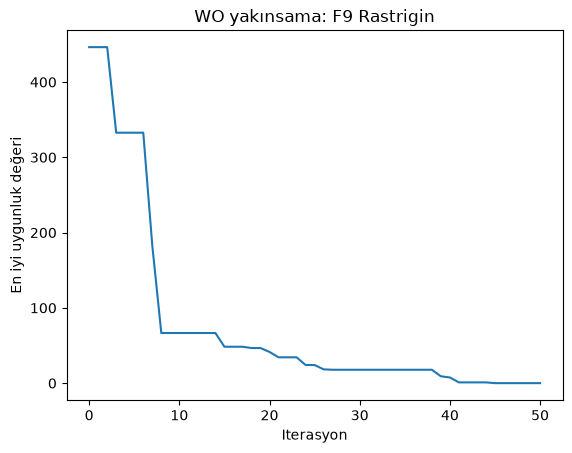
\includegraphics[width=\linewidth]{F9/convergence.png}
\end{minipage}\hfill
\begin{minipage}[t]{0.48\textwidth}\centering\small
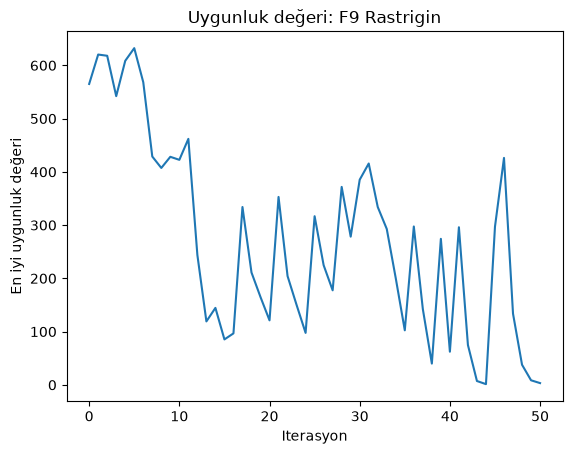
\includegraphics[width=\linewidth]{F9/average_fitness.png}
\end{minipage}
\caption{WO'nun F9 Rastrigin fonksiyonundaki nitel arama sonuçları.}
\label{fig:wo-f9-qualitative}
\end{figure}

F9 Rastrigin çok sayıda yerel optimum içerir. Şekil~\ref{fig:wo-f9-qualitative}'de noktaların geniş bir alana yayıldıktan sonra orijin çevresinde de yoğunlaştığı görülür. Yakınsama eğrisi en iyi değerin yinelemeler ilerledikçe kademeli olarak azaldığını ve çalıştırmanın son bölümünde sıfıra yaklaştığını gösterir. İlk morsun yörüngesi ve ortalama uygunluk eğrisi ise büyük sıçramalar ve dalgalanmalar sergiler. Bu nedenle arama geçmişindeki merkezî yoğunlaşma, her ajanın yerel optimumlardan kaçtığını tek başına kanıtlamaz.

\begin{figure}[htbp]
\centering
\begin{minipage}[t]{0.48\textwidth}\centering\small
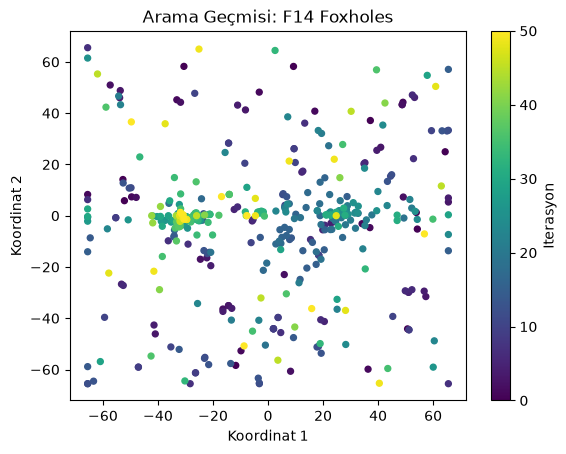
\includegraphics[width=\linewidth]{F14/search_history.png}
\end{minipage}\hfill
\begin{minipage}[t]{0.48\textwidth}\centering\small
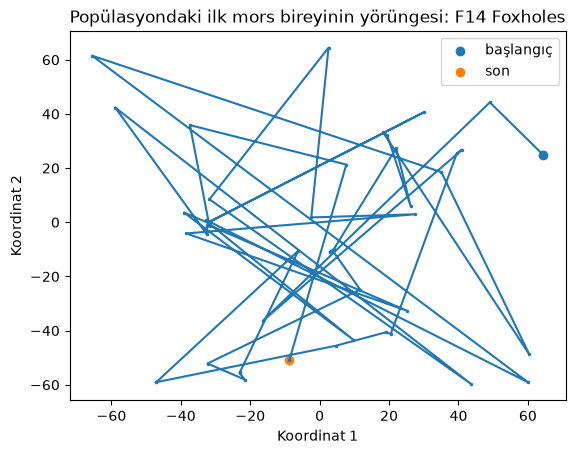
\includegraphics[width=\linewidth]{F14/first_walrus_trajectory.png}
\end{minipage}\par\medskip
\begin{minipage}[t]{0.48\textwidth}\centering\small
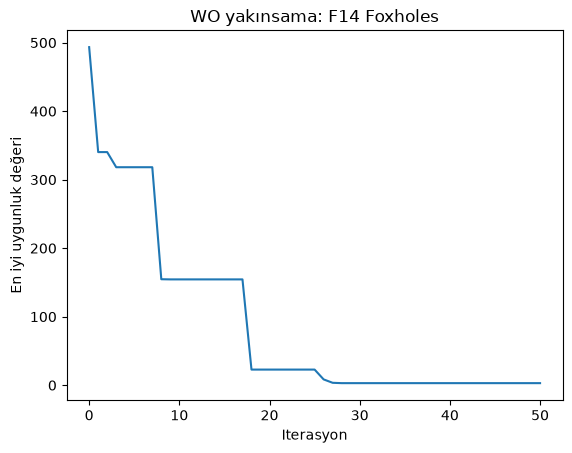
\includegraphics[width=\linewidth]{F14/convergence.png}
\end{minipage}\hfill
\begin{minipage}[t]{0.48\textwidth}\centering\small
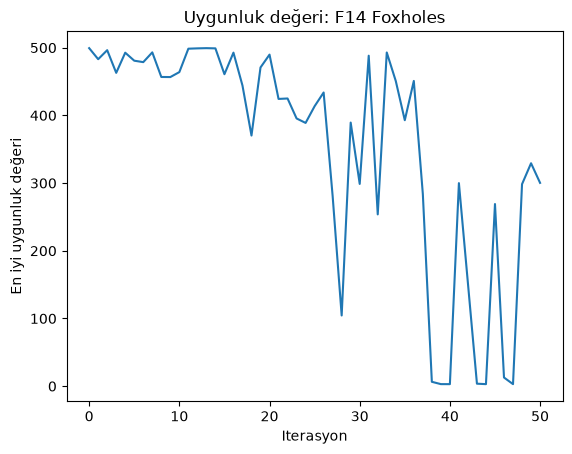
\includegraphics[width=\linewidth]{F14/average_fitness.png}
\end{minipage}
\caption{WO'nun F14 Foxholes fonksiyonundaki nitel arama sonuçları.}
\label{fig:wo-f14-qualitative}
\end{figure}

Şekil~\ref{fig:wo-f14-qualitative}’te, F14 Foxholes için arama geçmişi, ajanların arama uzayının geniş bir bölümünü ziyaret ettiğini ve bazı 
bölgelerde kümelenmeler oluştuğunu göstermektedir. İlk morsun yörüngesi geniş ve düzensiz hareketler içerir; 
başlangıç noktası yaklaşık \((65,25)\), son noktası ise yaklaşık \((-9,-50)\)’dir. Bu yörünge, ilk morsun optimuma 
yakınsadığını göstermemektedir. Buna karşılık yakınsama eğrisi, bulunan en iyi uygunluk değerinin ilk yaklaşık 
27 yinelemede belirgin biçimde azaldığını ve sonrasında sıfıra yakın kaldığını göstermektedir. Popülasyonun uygunluk 
değerindeki büyük dalgalanmalar ise bireylerin aynı hızda kararlı hâle gelmediğine işaret eder. Dolayısıyla en iyi 
çözümün hızla iyileşmesi, ilk morsun veya popülasyonun tamamının optimuma yakınsadığı anlamına gelmez.

Han ve arkadaşları makaledeki seçili testlerde, yinelemeler ilerledikçe ilk ajanın hareket genliğinin azaldığını, 
aramanın daha elverişli bölgelere yöneldiğini ve ortalama uygunluğun düştüğünü bildirmiştir \cite{han2024walrus}. 
Buradaki grafiklerde en iyi çözüm eğrileri bu iyileşme eğilimiyle uyumludur; ancak ilk morsun yörüngeleri ve 
popülasyon ortalaması her üç fonksiyonda da belirgin hareketlilik göstermektedir.

\subsection{Nicel analiz}

\paragraph{Toplu karşılaştırma.}
Her fonksiyon için 100 çalıştırmanın ortalama uygunluk değerleri esas alınarak
algoritmalar sıralanmıştır. Buna göre WO, POS'u 23 fonksiyonun 16'sında, ACO'yu
ise 15'inde geçmiştir. ACO da POS'tan 18 fonksiyonda daha düşük ortalama
uygunluk elde etmiştir. Tablo~\ref{tab:overall-rank-results}, ortalama uygunluk
temelindeki ikili W/T/L sonuçlarını göstermektedir.

\begin{table}[htbp]
\centering
\small
\caption{Ortalama uygunluk değerlerine göre ikili W/T/L sonuçları ve Friedman ortalama sıra değerleri.}
\label{tab:overall-rank-results}
\begin{tabular}{@{}lrrrr@{}}
\hline
\textbf{Karşılaştırma} & \textbf{W} & \textbf{T} & \textbf{L} & \textbf{Fonksiyon sayısı} \\
\hline
WO--POS & 16 & 0 & 7 & 23 \\
WO--ACO & 15 & 0 & 8 & 23 \\
ACO--POS & 18 & 0 & 5 & 23 \\
\hline
\end{tabular}
\vspace{0.8em}
\begin{tabular}{@{}lrr@{}}
\hline
\textbf{Algoritma} & \textbf{Friedman ortalama sırası} & \textbf{Genel sıra} \\
\hline
WO & 1.652 & 1 \\
ACO & 1.870 & 2 \\
POS & 2.478 & 3 \\
\hline
\end{tabular}
\end{table}
Friedman testi, algoritmalar arasında genel bir fark bulunduğunu göstermiştir ($\chi^2(2)=8.435$, $p=0.0147$). Friedman testi ikili farkları tek başına belirlemediğinden, algoritma çiftleri için post-hoc test yapılmadan ikili istatistiksel anlamlılık iddiasında bulunulmamıştır.


\small
\setlength{\tabcolsep}{3pt}
\renewcommand{\arraystretch}{1.12}
\begin{longtable}{@{}p{2.25cm}p{4.25cm}p{4.25cm}p{4.25cm}@{}}
\caption{WO, POS ve ACO algoritmalarının 23 kıyaslama fonksiyonundaki sonuçları. Süreler 100 çalıştırmadaki medyan saniye değeridir.}\label{tab:all-benchmark-results}\\
\hline
\textbf{Fonksiyon} & \textbf{WO} & \textbf{POS} & \textbf{ACO} \\
\hline
\endfirsthead
\multicolumn{4}{c}{\tablename\ \thetable{} -- devamı}\\
\hline
\textbf{Fonksiyon} & \textbf{WO} & \textbf{POS} & \textbf{ACO} \\
\hline
\endhead
\hline
\multicolumn{4}{r}{Devamı sonraki sayfada}\\
\endfoot
\hline
\endlastfoot
\multicolumn{4}{@{}l}{\textbf{Tek tepeli fonksiyonlar (F1--F7)}}\\
F1 Sphere & \makecell[l]{En iyi: $4.794\times 10^{-10}$\\ En kötü: $96.65$\\ Ortalama: $3.078$\\ Std. sapma: $12.42$\\ Medyan süre: $0.01379\,\mathrm{s}$} & \makecell[l]{En iyi: $1.725\times 10^{4}$\\ En kötü: $5.567\times 10^{4}$\\ Ortalama: $3.67\times 10^{4}$\\ Std. sapma: $8553$\\ Medyan süre: $0.005513\,\mathrm{s}$} & \makecell[l]{En iyi: $2771$\\ En kötü: $2.069\times 10^{4}$\\ Ortalama: $1.128\times 10^{4}$\\ Std. sapma: $3735$\\ Medyan süre: $0.01193\,\mathrm{s}$} \\
F2 Schwefel 2.22 & \makecell[l]{En iyi: $7.989\times 10^{-7}$\\ En kötü: $2.772$\\ Ortalama: $0.2129$\\ Std. sapma: $0.4244$\\ Medyan süre: $0.01567\,\mathrm{s}$} & \makecell[l]{En iyi: $90.45$\\ En kötü: $2.192\times 10^{9}$\\ Ortalama: $8.319\times 10^{7}$\\ Std. sapma: $3.658\times 10^{8}$\\ Medyan süre: $0.008007\,\mathrm{s}$} & \makecell[l]{En iyi: $26.93$\\ En kötü: $6441$\\ Ortalama: $185.4$\\ Std. sapma: $711.3$\\ Medyan süre: $0.01178\,\mathrm{s}$} \\
F3 Schwefel 1.2 & \makecell[l]{En iyi: $3.204\times 10^{-9}$\\ En kötü: $9740$\\ Ortalama: $237.8$\\ Std. sapma: $1125$\\ Medyan süre: $0.008233\,\mathrm{s}$} & \makecell[l]{En iyi: $4.442\times 10^{4}$\\ En kötü: $1.24\times 10^{5}$\\ Ortalama: $7.943\times 10^{4}$\\ Std. sapma: $1.84\times 10^{4}$\\ Medyan süre: $0.003734\,\mathrm{s}$} & \makecell[l]{En iyi: $4.152\times 10^{4}$\\ En kötü: $1.22\times 10^{5}$\\ Ortalama: $7.589\times 10^{4}$\\ Std. sapma: $1.631\times 10^{4}$\\ Medyan süre: $0.006859\,\mathrm{s}$} \\
F4 Schwefel 2.21 & \makecell[l]{En iyi: $1.504\times 10^{-7}$\\ En kötü: $11.28$\\ Ortalama: $0.7973$\\ Std. sapma: $1.714$\\ Medyan süre: $0.006398\,\mathrm{s}$} & \makecell[l]{En iyi: $66.54$\\ En kötü: $96.86$\\ Ortalama: $88.51$\\ Std. sapma: $5.607$\\ Medyan süre: $0.002547\,\mathrm{s}$} & \makecell[l]{En iyi: $73.54$\\ En kötü: $96.86$\\ Ortalama: $90.94$\\ Std. sapma: $4.142$\\ Medyan süre: $0.005817\,\mathrm{s}$} \\
F5 Rosenbrock & \makecell[l]{En iyi: $28.95$\\ En kötü: $1.056\times 10^{5}$\\ Ortalama: $1127$\\ Std. sapma: $1.056\times 10^{4}$\\ Medyan süre: $0.008323\,\mathrm{s}$} & \makecell[l]{En iyi: $2.617\times 10^{7}$\\ En kötü: $2.649\times 10^{8}$\\ Ortalama: $9.89\times 10^{7}$\\ Std. sapma: $4.607\times 10^{7}$\\ Medyan süre: $0.00439\,\mathrm{s}$} & \makecell[l]{En iyi: $1.88\times 10^{6}$\\ En kötü: $7.884\times 10^{7}$\\ Ortalama: $2.912\times 10^{7}$\\ Std. sapma: $1.57\times 10^{7}$\\ Medyan süre: $0.007724\,\mathrm{s}$} \\
F6 Step & \makecell[l]{En iyi: $0$\\ En kötü: $42$\\ Ortalama: $2.5$\\ Std. sapma: $7.132$\\ Medyan süre: $0.007244\,\mathrm{s}$} & \makecell[l]{En iyi: $1.712\times 10^{4}$\\ En kötü: $6.123\times 10^{4}$\\ Ortalama: $3.575\times 10^{4}$\\ Std. sapma: $8683$\\ Medyan süre: $0.003149\,\mathrm{s}$} & \makecell[l]{En iyi: $3249$\\ En kötü: $2.34\times 10^{4}$\\ Ortalama: $1.181\times 10^{4}$\\ Std. sapma: $3561$\\ Medyan süre: $0.006282\,\mathrm{s}$} \\
F7 Quartic & \makecell[l]{En iyi: $0.005393$\\ En kötü: $4.336\times 10^{5}$\\ Ortalama: $4633$\\ Std. sapma: $4.337\times 10^{4}$\\ Medyan süre: $0.009031\,\mathrm{s}$} & \makecell[l]{En iyi: $7.385\times 10^{8}$\\ En kötü: $8.591\times 10^{9}$\\ Ortalama: $4.258\times 10^{9}$\\ Std. sapma: $1.681\times 10^{9}$\\ Medyan süre: $0.004956\,\mathrm{s}$} & \makecell[l]{En iyi: $3.154\times 10^{8}$\\ En kötü: $3.779\times 10^{9}$\\ Ortalama: $1.272\times 10^{9}$\\ Std. sapma: $6.532\times 10^{8}$\\ Medyan süre: $0.008021\,\mathrm{s}$} \\
\multicolumn{4}{@{}l}{\textbf{Çok tepeli fonksiyonlar (F8--F13)}}\\
F8 Schwefel 2.26 & \makecell[l]{En iyi: $-7789$\\ En kötü: $-2134$\\ Ortalama: $-3460$\\ Std. sapma: $928.5$\\ Medyan süre: $0.007317\,\mathrm{s}$} & \makecell[l]{En iyi: $-7344$\\ En kötü: $-4190$\\ Ortalama: $-5726$\\ Std. sapma: $715.7$\\ Medyan süre: $0.003529\,\mathrm{s}$} & \makecell[l]{En iyi: $-5105$\\ En kötü: $-2390$\\ Ortalama: $-3392$\\ Std. sapma: $559.3$\\ Medyan süre: $0.006649\,\mathrm{s}$} \\
F9 Rastrigin & \makecell[l]{En iyi: $3.675\times 10^{-9}$\\ En kötü: $146$\\ Ortalama: $2.879$\\ Std. sapma: $15.5$\\ Medyan süre: $0.007749\,\mathrm{s}$} & \makecell[l]{En iyi: $288$\\ En kötü: $451$\\ Ortalama: $375.9$\\ Std. sapma: $36.58$\\ Medyan süre: $0.003985\,\mathrm{s}$} & \makecell[l]{En iyi: $242.6$\\ En kötü: $413.7$\\ Ortalama: $324.3$\\ Std. sapma: $27.82$\\ Medyan süre: $0.007093\,\mathrm{s}$} \\
F10 Ackley & \makecell[l]{En iyi: $1.338\times 10^{-5}$\\ En kötü: $3.691$\\ Ortalama: $0.2538$\\ Std. sapma: $0.607$\\ Medyan süre: $0.01048\,\mathrm{s}$} & \makecell[l]{En iyi: $17.38$\\ En kötü: $20.68$\\ Ortalama: $20.1$\\ Std. sapma: $0.5688$\\ Medyan süre: $0.006594\,\mathrm{s}$} & \makecell[l]{En iyi: $12.35$\\ En kötü: $20.71$\\ Ortalama: $18.42$\\ Std. sapma: $1.916$\\ Medyan süre: $0.009975\,\mathrm{s}$} \\
F11 Griewank & \makecell[l]{En iyi: $1.181\times 10^{-10}$\\ En kötü: $11.63$\\ Ortalama: $0.561$\\ Std. sapma: $1.231$\\ Medyan süre: $0.009479\,\mathrm{s}$} & \makecell[l]{En iyi: $128.7$\\ En kötü: $531.7$\\ Ortalama: $320$\\ Std. sapma: $77.4$\\ Medyan süre: $0.005419\,\mathrm{s}$} & \makecell[l]{En iyi: $52.5$\\ En kötü: $220.4$\\ Ortalama: $106.5$\\ Std. sapma: $31.11$\\ Medyan süre: $0.008727\,\mathrm{s}$} \\
F12 Penalized 1 & \makecell[l]{En iyi: $0.1766$\\ En kötü: $5.392$\\ Ortalama: $1.157$\\ Std. sapma: $0.5741$\\ Medyan süre: $0.01374\,\mathrm{s}$} & \makecell[l]{En iyi: $2.866\times 10^{7}$\\ En kötü: $5.203\times 10^{8}$\\ Ortalama: $1.879\times 10^{8}$\\ Std. sapma: $9.329\times 10^{7}$\\ Medyan süre: $0.009702\,\mathrm{s}$} & \makecell[l]{En iyi: $4.059\times 10^{6}$\\ En kötü: $3.828\times 10^{8}$\\ Ortalama: $7.592\times 10^{7}$\\ Std. sapma: $6.763\times 10^{7}$\\ Medyan süre: $0.0133\,\mathrm{s}$} \\
F13 Penalized 2 & \makecell[l]{En iyi: $2.369$\\ En kötü: $50.6$\\ Ortalama: $3.915$\\ Std. sapma: $4.902$\\ Medyan süre: $0.0126\,\mathrm{s}$} & \makecell[l]{En iyi: $7.835\times 10^{7}$\\ En kötü: $1.176\times 10^{9}$\\ Ortalama: $3.999\times 10^{8}$\\ Std. sapma: $2.215\times 10^{8}$\\ Medyan süre: $0.008618\,\mathrm{s}$} & \makecell[l]{En iyi: $1.806\times 10^{7}$\\ En kötü: $6.201\times 10^{8}$\\ Ortalama: $1.528\times 10^{8}$\\ Std. sapma: $1.018\times 10^{8}$\\ Medyan süre: $0.01188\,\mathrm{s}$} \\
\multicolumn{4}{@{}l}{\textbf{Sabit boyutlu çok tepeli fonksiyonlar (F14--F23)}}\\
F14 Foxholes & \makecell[l]{En iyi: $0.998$\\ En kötü: $16.44$\\ Ortalama: $6.535$\\ Std. sapma: $3.444$\\ Medyan süre: $0.00935\,\mathrm{s}$} & \makecell[l]{En iyi: $0.998$\\ En kötü: $20.21$\\ Ortalama: $3.849$\\ Std. sapma: $3.865$\\ Medyan süre: $0.006552\,\mathrm{s}$} & \makecell[l]{En iyi: $0.998$\\ En kötü: $16.45$\\ Ortalama: $5.353$\\ Std. sapma: $3.605$\\ Medyan süre: $0.009232\,\mathrm{s}$} \\
F15 Kowalik & \makecell[l]{En iyi: $0.00592$\\ En kötü: $0.1316$\\ Ortalama: $0.03691$\\ Std. sapma: $0.02265$\\ Medyan süre: $0.008102\,\mathrm{s}$} & \makecell[l]{En iyi: $0.005437$\\ En kötü: $0.1285$\\ Ortalama: $0.0585$\\ Std. sapma: $0.03518$\\ Medyan süre: $0.005234\,\mathrm{s}$} & \makecell[l]{En iyi: $0.004373$\\ En kötü: $0.09887$\\ Ortalama: $0.02601$\\ Std. sapma: $0.02265$\\ Medyan süre: $0.008094\,\mathrm{s}$} \\
F16 Six-hump Camel & \makecell[l]{En iyi: $-1.032$\\ En kötü: $-0.9906$\\ Ortalama: $-1.028$\\ Std. sapma: $0.00759$\\ Medyan süre: $0.004477\,\mathrm{s}$} & \makecell[l]{En iyi: $-1.032$\\ En kötü: $-1.026$\\ Ortalama: $-1.031$\\ Std. sapma: $0.0007045$\\ Medyan süre: $0.001905\,\mathrm{s}$} & \makecell[l]{En iyi: $-1.032$\\ En kötü: $-0.2155$\\ Ortalama: $-1.023$\\ Std. sapma: $0.08161$\\ Medyan süre: $0.00468\,\mathrm{s}$} \\
F17 Branin & \makecell[l]{En iyi: $0.3979$\\ En kötü: $0.6619$\\ Ortalama: $0.4146$\\ Std. sapma: $0.04435$\\ Medyan süre: $0.004559\,\mathrm{s}$} & \makecell[l]{En iyi: $0.3979$\\ En kötü: $12.72$\\ Ortalama: $0.6505$\\ Std. sapma: $1.522$\\ Medyan süre: $0.002001\,\mathrm{s}$} & \makecell[l]{En iyi: $0.3979$\\ En kötü: $0.3979$\\ Ortalama: $0.3979$\\ Std. sapma: $4.873\times 10^{-7}$\\ Medyan süre: $0.004659\,\mathrm{s}$} \\
F18 Goldstein-Price & \makecell[l]{En iyi: $3$\\ En kötü: $3.993$\\ Ortalama: $3.107$\\ Std. sapma: $0.184$\\ Medyan süre: $0.005224\,\mathrm{s}$} & \makecell[l]{En iyi: $3$\\ En kötü: $84.94$\\ Ortalama: $11.56$\\ Std. sapma: $24.66$\\ Medyan süre: $0.002675\,\mathrm{s}$} & \makecell[l]{En iyi: $3$\\ En kötü: $86.1$\\ Ortalama: $8.591$\\ Std. sapma: $17.84$\\ Medyan süre: $0.005251\,\mathrm{s}$} \\
F19 Hartmann 3D & \makecell[l]{En iyi: $-3.862$\\ En kötü: $-2.986$\\ Ortalama: $-3.768$\\ Std. sapma: $0.1447$\\ Medyan süre: $0.008336\,\mathrm{s}$} & \makecell[l]{En iyi: $-3.863$\\ En kötü: $-2.664$\\ Ortalama: $-3.816$\\ Std. sapma: $0.1672$\\ Medyan süre: $0.005525\,\mathrm{s}$} & \makecell[l]{En iyi: $-3.863$\\ En kötü: $-1.001$\\ Ortalama: $-3.834$\\ Std. sapma: $0.2862$\\ Medyan süre: $0.008116\,\mathrm{s}$} \\
F20 Hartmann 6D & \makecell[l]{En iyi: $-3.307$\\ En kötü: $-2.194$\\ Ortalama: $-3.108$\\ Std. sapma: $0.1753$\\ Medyan süre: $0.008287\,\mathrm{s}$} & \makecell[l]{En iyi: $-3.322$\\ En kötü: $-1.255$\\ Ortalama: $-3.039$\\ Std. sapma: $0.4329$\\ Medyan süre: $0.005498\,\mathrm{s}$} & \makecell[l]{En iyi: $-3.322$\\ En kötü: $-3.191$\\ Ortalama: $-3.277$\\ Std. sapma: $0.05792$\\ Medyan süre: $0.008248\,\mathrm{s}$} \\
F21 Shekel 5 & \makecell[l]{En iyi: $-9.559$\\ En kötü: $-1.73$\\ Ortalama: $-4.558$\\ Std. sapma: $1.557$\\ Medyan süre: $0.009906\,\mathrm{s}$} & \makecell[l]{En iyi: $-10.14$\\ En kötü: $-0.4973$\\ Ortalama: $-5.507$\\ Std. sapma: $3.252$\\ Medyan süre: $0.007176\,\mathrm{s}$} & \makecell[l]{En iyi: $-10.15$\\ En kötü: $-2.196$\\ Ortalama: $-5.276$\\ Std. sapma: $3.529$\\ Medyan süre: $0.009805\,\mathrm{s}$} \\
F22 Shekel 7 & \makecell[l]{En iyi: $-10.13$\\ En kötü: $-1.957$\\ Ortalama: $-4.403$\\ Std. sapma: $1.216$\\ Medyan süre: $0.009915\,\mathrm{s}$} & \makecell[l]{En iyi: $-10.4$\\ En kötü: $-0.9116$\\ Ortalama: $-4.93$\\ Std. sapma: $3.078$\\ Medyan süre: $0.007203\,\mathrm{s}$} & \makecell[l]{En iyi: $-10.4$\\ En kötü: $-1.838$\\ Ortalama: $-6.751$\\ Std. sapma: $3.695$\\ Medyan süre: $0.009829\,\mathrm{s}$} \\
F23 Shekel 10 & \makecell[l]{En iyi: $-10.12$\\ En kötü: $-1.718$\\ Ortalama: $-4.478$\\ Std. sapma: $1.651$\\ Medyan süre: $0.009745\,\mathrm{s}$} & \makecell[l]{En iyi: $-10.49$\\ En kötü: $-1.46$\\ Ortalama: $-4.733$\\ Std. sapma: $3.1$\\ Medyan süre: $0.007126\,\mathrm{s}$} & \makecell[l]{En iyi: $-10.54$\\ En kötü: $-1.809$\\ Ortalama: $-6.635$\\ Std. sapma: $3.9$\\ Medyan süre: $0.01003\,\mathrm{s}$} \\
\end{longtable}
\endgroup
